\begin{enumerate}
  \item Sea $R(m)$ el ingreso máximo que es posible obtener al partir un bloque de duración $m$ en pautas, para $m \in \{0, 1, \ldots, n\}$.

  \[
  R(m) =
  \begin{cases}
  0 & \text{si } m = 0 \\
  \max\limits_{1 \le i \le m} \big(\text{tarifa}[i] + R(m-i)\big) & \text{si } m > 0
  \end{cases}
  \]

  Símbolo por símbolo:
  \begin{itemize}
    \item $R(m)$: el ingreso máximo que se puede obtener al partir un bloque de duración $m$ en pautas.
    \item $R(n)$: el ingreso máximo que se puede obtener al partir un bloque de duración $n$ en pautas, es decir, la respuesta al problema.
    \item $m$: la duración del bloque que falta por repartir en pautas, entre $0$ y $n$.
    \item $i$: la duración de la primera pauta que se corta del bloque de tamaño $m$, entre $1$ y $m$.
    \item $\text{tarifa}[i]$: el precio de una pauta de duración $i$ (esto no es una variable).
    \item $\max$: prueba, para el bloque de tamaño $m$, cada duración posible $i$ de la primera pauta que se corta, y le suma el ingreso óptimo de repartir lo que queda ($m-i$). La mejor de esas $m$ opciones es $R(m)$.
  \end{itemize}

  \item Una tabulación de $R$ tiene una complejidad espacial de $\Theta(n)$: cada solución a un subproblema ocupa una entrada del arreglo.\\

  Examinando la recurrencia, es evidente que al computar $R(m)$ con \(m > 0\) se utilizan las soluciones de $R(0), \ldots, R(m-1)$. El grafo de dependencias es entonces el siguiente: 

\begin{center}
\setbox0=\hbox{%
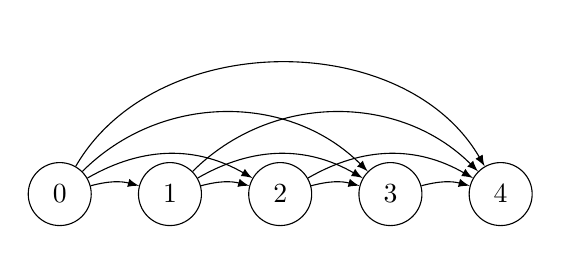
\begin{tikzpicture}[
  vertex/.style={circle, draw, minimum size=0.8cm, inner sep=0pt},
  -latex,
]
  \foreach \i in {0,...,4} {
    \node[vertex] (v\i) at (1.4*\i, 0) {\i};
  }

  \draw (v0) to[bend left=15] (v1);

  \draw (v0) to[bend left=30] (v2);
  \draw (v1) to[bend left=15] (v2);

  \draw (v0) to[bend left=45] (v3);
  \draw (v1) to[bend left=30] (v3);
  \draw (v2) to[bend left=15] (v3);

  \draw (v0) to[bend left=60] (v4);
  \draw (v1) to[bend left=45] (v4);
  \draw (v2) to[bend left=30] (v4);
  \draw (v3) to[bend left=15] (v4);
\end{tikzpicture}%
}
\ifdim\wd0>\textwidth
  \resizebox{\textwidth}{!}{\copy0}
\else
  \makebox[\linewidth]{\copy0}
\fi

\medskip
Grafo de dependencias de \(R(m)\) para \(n=4\).
\end{center}

  Se necesitan de todos los valores anteriores, por ende, no es posible optimizar el espacio por debajo de $\Theta(n)$, independientemente de si la implementación es top-down o bottom-up. \\

  También utilizando el grafo, es claro que resolver cada uno de los $n$ estados cuesta hasta $\Theta(n)$ trabajo (recorrer todos los vértices anteriores en el grafo, o recorrer el $\max$ en la relación de recurrencia). Ergo, la complejidad temporal es $\Theta(n^2)$: $\Theta(n)$ estados, cada uno con costo de $\Theta(n)$.

  \pagebreak

  \item Implementaciones top-down y bottom up en Python. Ambas con complejidad espacial $\Theta(n)$ y complejidad temporal $\Theta(n^2)$.

\begin{pseudocode}
def max_ingreso_top_down(tarifa: list[int]) -> int:
    n = len(tarifa) - 1
    ingreso = [None] * (n + 1)
    ingreso[0] = 0

    return max_ingreso_memo(n, tarifa, ingreso)

def max_ingreso_memo(m: int, tarifa: list[int], ingreso: list[int]) -> int:
    if ingreso[m] is not None:
        return ingreso[m]

    mejor = 0
    for i in range(1, m + 1):
        mejor = max(mejor, tarifa[i] + max_ingreso_memo(m - i, tarifa, ingreso))

    ingreso[m] = mejor
    return mejor
\end{pseudocode}

\begin{pseudocode}
def max_ingreso_bottom_up(tarifa: list[int]) -> int:
    n = len(tarifa) - 1
    ingreso = [0] * (n + 1)

    for m in range(1, n + 1):
        mejor = 0
        for i in range(1, m + 1):
            mejor = max(mejor, tarifa[i] + ingreso[m - i])
        ingreso[m] = mejor

    return ingreso[n]
\end{pseudocode}
\end{enumerate}
